\begin{figure}
\centering

\begin{subfigure}{0.45\textwidth}
  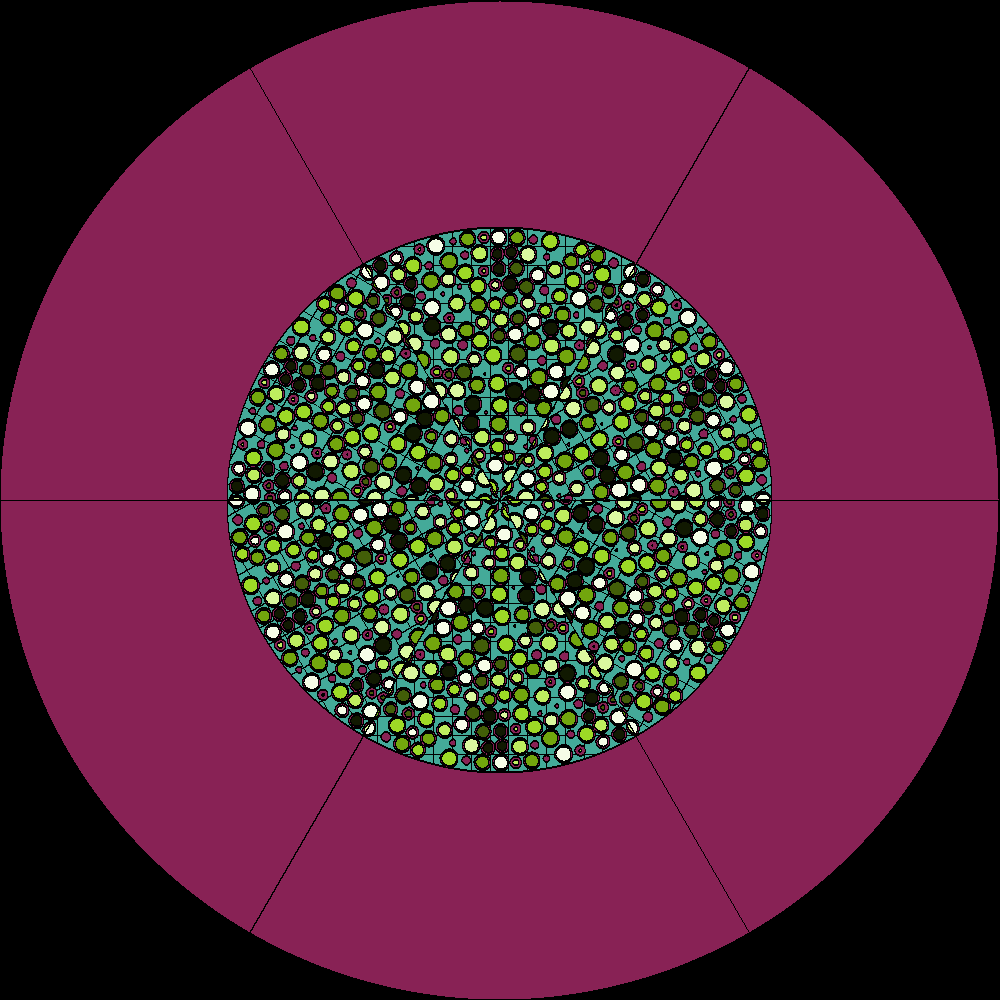
\includegraphics[width=0.95\linewidth]{figures/60-120/60-120-r}
  \caption{Radial Cross Section at y=0}
  \label{fig:bstep0}
\end{subfigure}%
%
\begin{subfigure}{0.45\textwidth}
  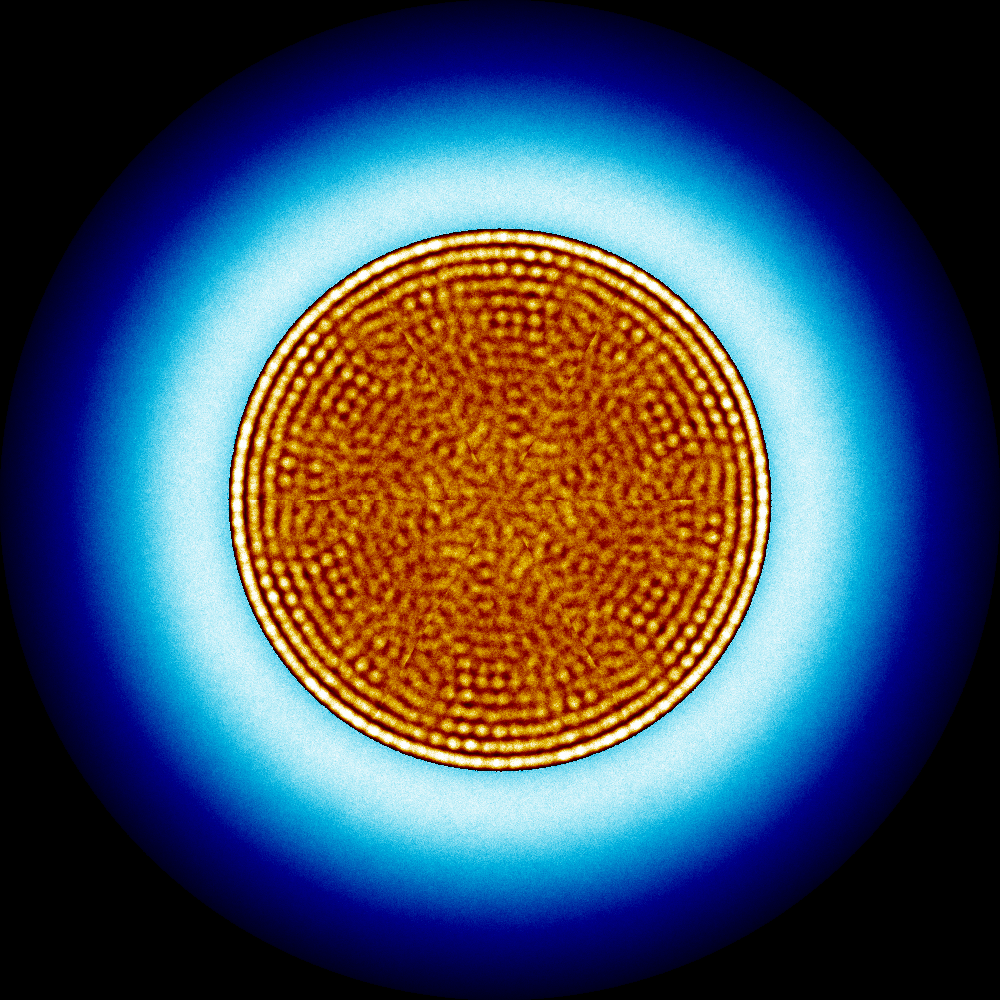
\includegraphics[width=0.95\linewidth]{figures/60-120/60-120-rm}
  \caption{Radial Mesh}
  \label{fig:bstep1}
\end{subfigure}

\begin{subfigure}{0.45\textwidth}
  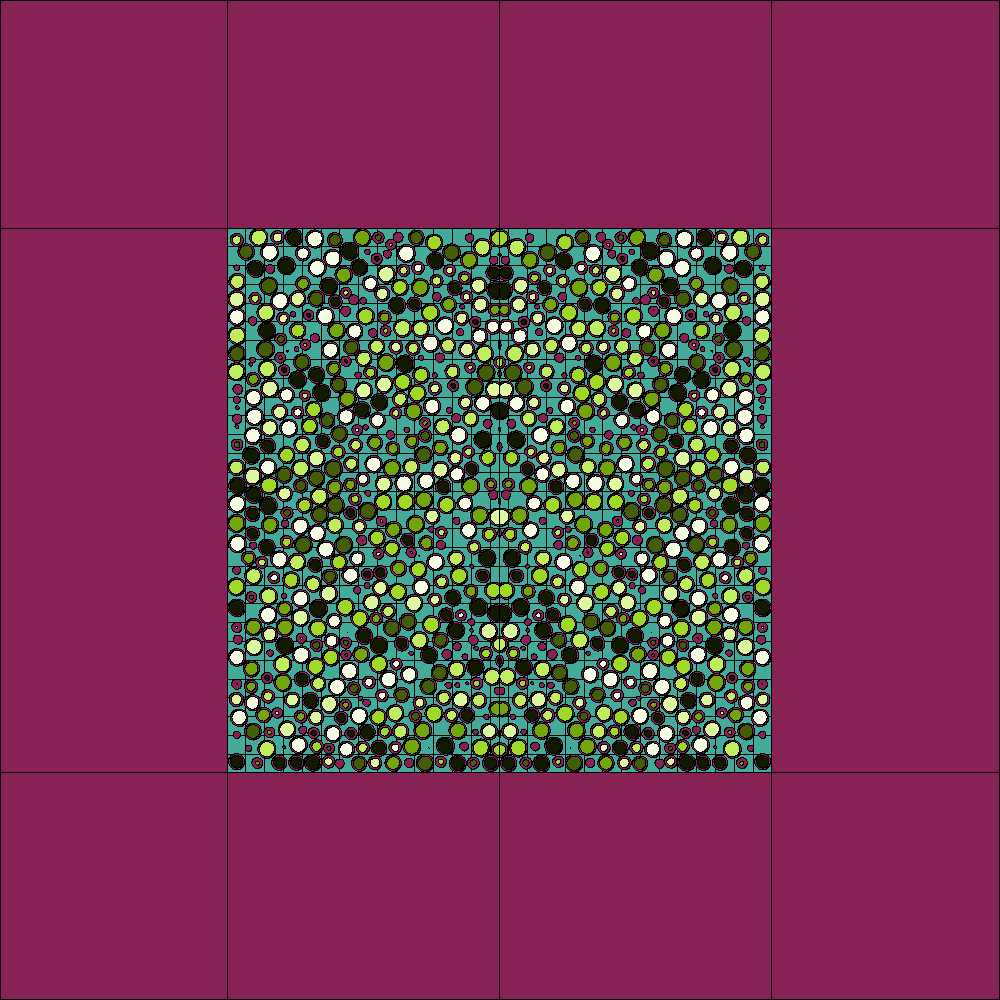
\includegraphics[width=0.95\linewidth]{figures/60-120/60-120-v}
  \caption{Axial Cross Section at z=0 }
  \label{fig:bstep1}
\end{subfigure}
%
\begin{subfigure}{0.45\textwidth}
  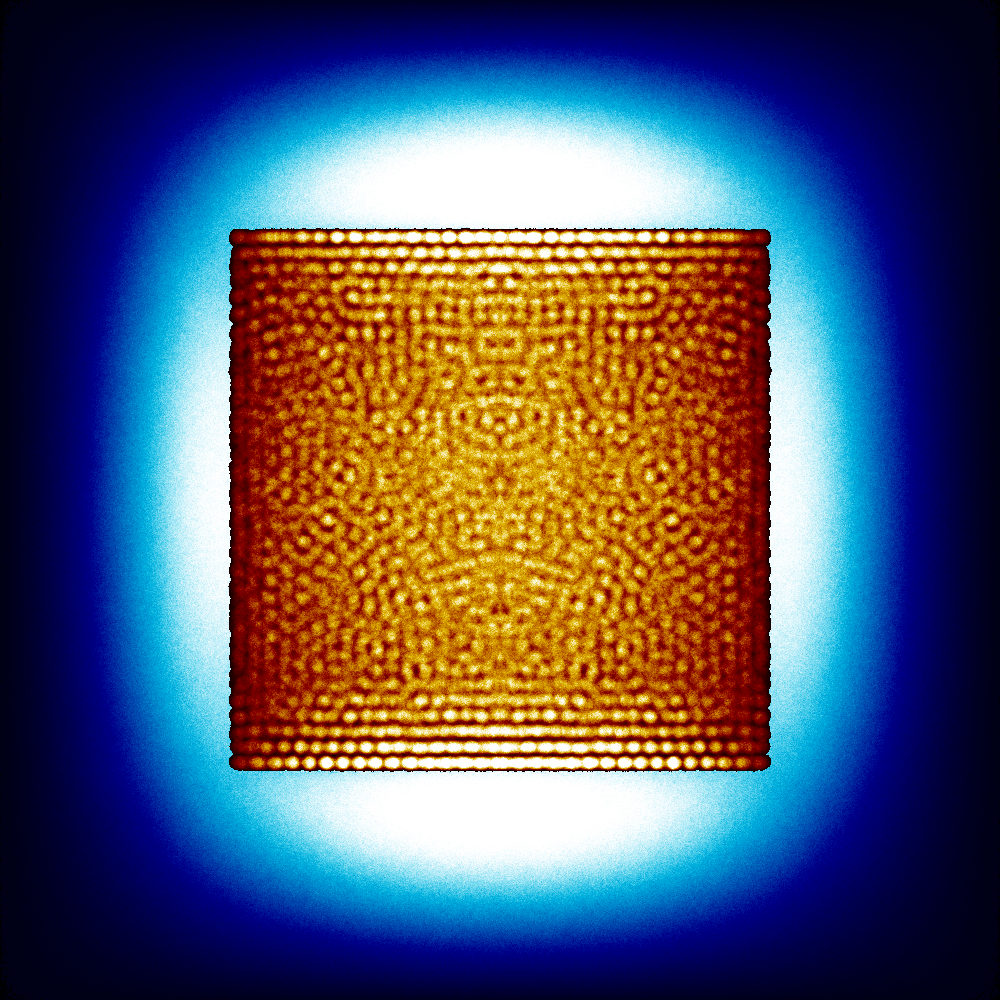
\includegraphics[width=0.95\linewidth]{figures/60-120/60-120-vm}
  \caption{Axial Mesh}
  \label{fig:bstep1}
\end{subfigure}
%
\caption{Sensitivity Analysis: $60^{\circ}$ - $120^{\circ}$}
\label{fig:60-120}
\end{figure}